\chapter{RESULTADOS E DISCUSSÃO}

Neste item será apresentado tudo que foi desenvolvido no presente trabalho.

\section{FERRAMENTA COMPUTACIONAL D'ÁGUA}

As páginas da interface gráfica ficaram divididas entre as abas iniciais, e a barra de ferramentas.

\subsection{As abas da ferramenta}

A interface gráfica ficou dividida em três abas. A primeira e principal delas têm o nome de \textbf{Equações do Mapa} e mostra o mapa interativo da Paraíba, que como explicado anteriormente, permite o cálculo da equação IDF através da escolha de uma coordenada ao clicar no mapa, por meio de interpolação. Também é possível apenas escolher uma das cidades paraibanas contida na lista. Tudo isso pode ser visto na Figura 5.1.\bigskip

\begin{figure}[!ht]
	\centering
	\caption{Aba "Equações do Mapa".}
	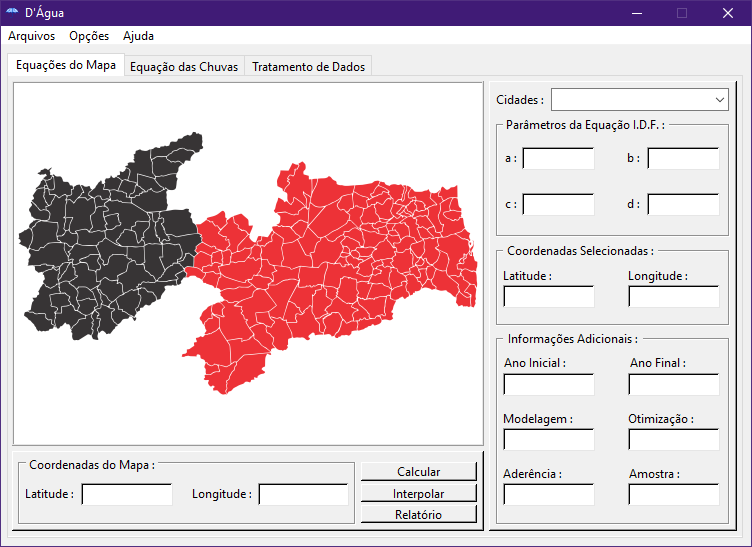
\includegraphics[width=.7625\linewidth]{figuras/equacoes_do_mapa.png}
	\caption*{\textbf{Fonte:} De autoria própria (2023).}
	\label{fig:equacoes_do_mapa.png}
\end{figure}

 A segunda aba é chamada de \textbf{Equações das Chuvas} e envolve os cálculos da equação IDF com base nos dados de séries temporais inseridos pelo usuário. Nela também é possível configurar as durações, tempos de retorno e métodos usados tanto nos cálculos citados anteriormente, como nos da primeira aba que utilizam as precipitações do banco de dados. Ou seja, suas configurações afetam toda a ferramenta e podem ser vistas na Figura 5.2.

\begin{figure}[!ht]
	\centering
	\caption{Aba "Gerador de Equações".}
	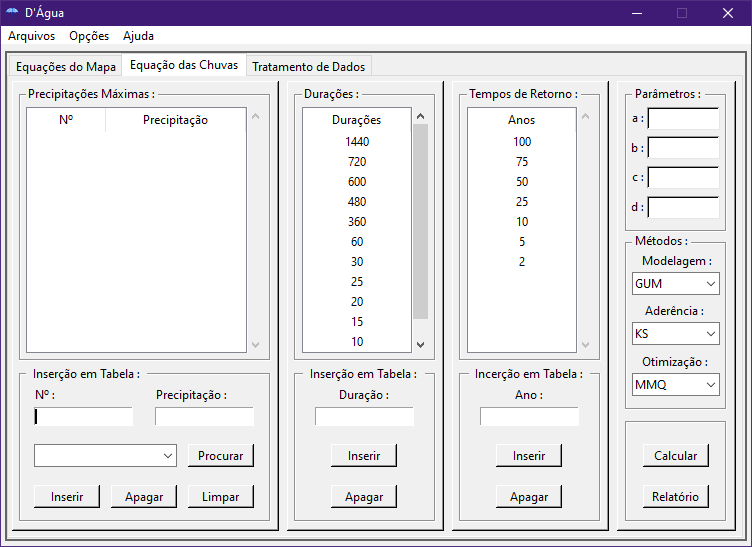
\includegraphics[width=.7625\linewidth]{figuras/equacoes_das_chuvas.png}
	\caption*{\textbf{Fonte:} De autoria própria (2023).}
	\label{fig:equacoes_das_chuvas.png}
\end{figure}

Observa-se a terceira e última aba na Figura 5.3, chamada de \textbf{Tratamento de Dados}, ela envolve o tratamento de séries históricas de precipitações diárias, resultando nas máximas diárias anuais, que podem ser exportadas para o cálculo da equação IDF na segunda aba.\bigskip

\begin{figure}[!ht]
	\centering
	\caption{Aba "Opções das Equações".}
	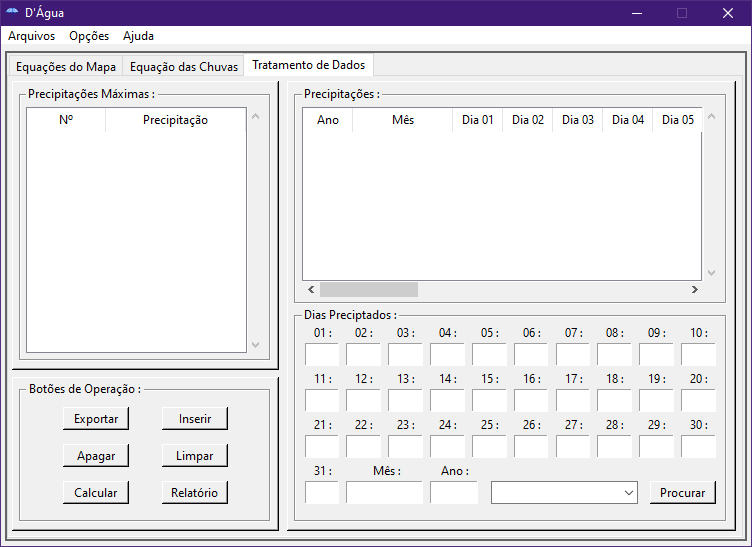
\includegraphics[width=.7625\linewidth]{figuras/tratamento_de_dados.png}
	\caption*{\textbf{Fonte:} De autoria própria (2023).}
	\label{fig:tratamento_de_dados.png}
\end{figure}

\newpage

\subsection{A barra de ferramentas}

A primeira ferramenta da barra é chama \textbf{Arquivos}, e nela há a possibilidade de reiniciar ou apenas sair do programa. Já em \textbf{Opções} é possível acessar o banco de dados, as configurações e as varreduras.

O banco de dados contém as informações de precipitações diárias das cidades da Paraíba, que são usados no desenvolvimento do método de preenchimento de falhas por interpolação IDW nos cálculos do mapa paraibano e da lista de cidades. Também é possível exportar os dados da cidade escolhida para a aba de tratamento de dados ou salva-los na própria máquina do usuário, no formato \textit{Comma-Separated-Values} (CSV).\bigskip

\begin{figure}[!ht]
	\centering
	\caption{Banco de dados da ferramenta Opções.}
	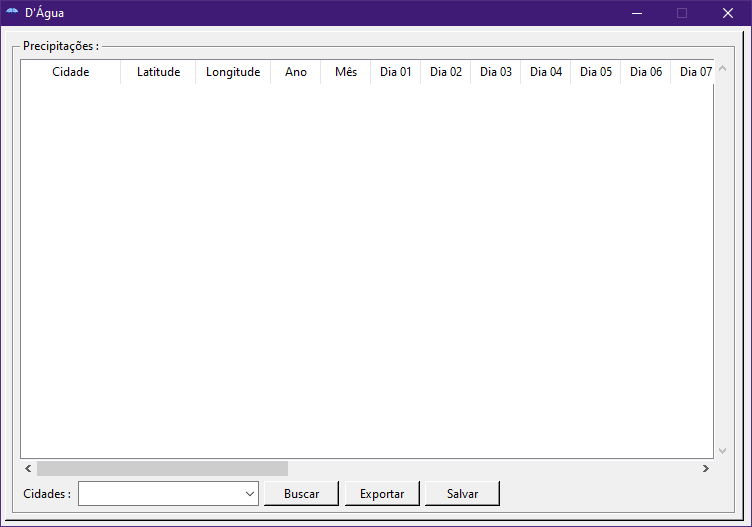
\includegraphics[width=.7625\linewidth]{figuras/banco_de_dados.png}
	\caption*{\textbf{Fonte:} De autoria própria (2023).}
	\label{fig:banco_de_dados.png}
\end{figure}

Já a ferramenta configurações possibilita ao usuário definir manualmente algumas informações que são usadas nos cálculos presentes na ferramenta. Seguindo pela ordem, é possível escolher entre coeficientes próprios de desagregação ou os estabelecidos pela DAEE/CETESB (1980), e a porcentagem de aderência usada no cálculo da equação IDF.

Também é possível decidir a quantidade de dias que representará o limiar de falhas usado na terceira aba, as otimizações de modelagem, aderência e otimização que caso ativados buscarão sempre os métodos que resultam em mais precisão nos parâmetros da equação IDF gerada. Por fim há a possibilidade de escolher a quantidade de iteração que o algoritmo fará durante o uso dos métodos de otimização no cálculo dos parâmetros da equação. É importante salientar que o mal uso dessas ferramentas pode exigir altos níveis de processamento da máquina devido a grande quantidade de iterações. É possível Observar na Figura 5.5 a página de configurações.

\newpage

\begin{figure}[!ht]
	\centering
	\caption{Configurações da ferramenta Opções.}
	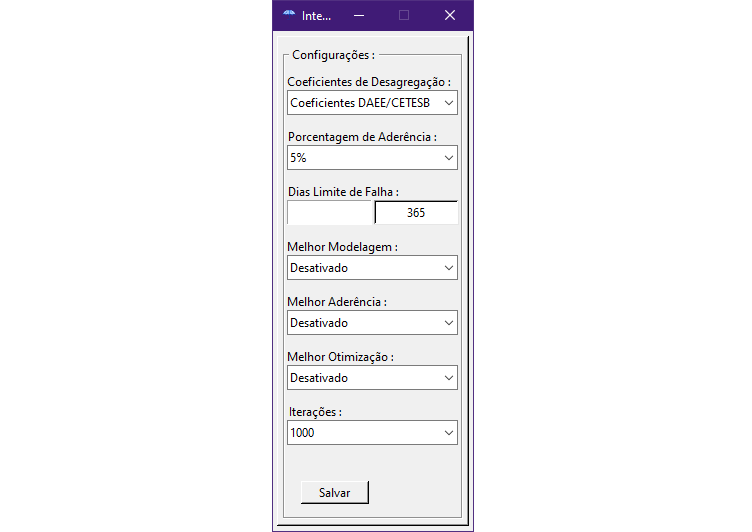
\includegraphics[width=.7625\linewidth]{figuras/configuracoes.png}
	\caption*{\textbf{Fonte:} De autoria própria (2023).}
	\label{fig:figuras/configuracoes.png}
\end{figure}

A ferramenta varreduras pode ser vista na Figura 5.6. Ela permite ao usuário alterar os números de partida ou intervalos dos métodos de otimização. Bons ajustes manuais dos mesmos pode resultar em uma melhora na precisão das equações geradas, em contrapartida o mal uso pode diminuir as porcentagens de acurácia ou até mesmo inviabilizar a o cálculo.\bigskip

\begin{figure}[!ht]
	\centering
	\caption{Varreduras da ferramenta Opções.}
	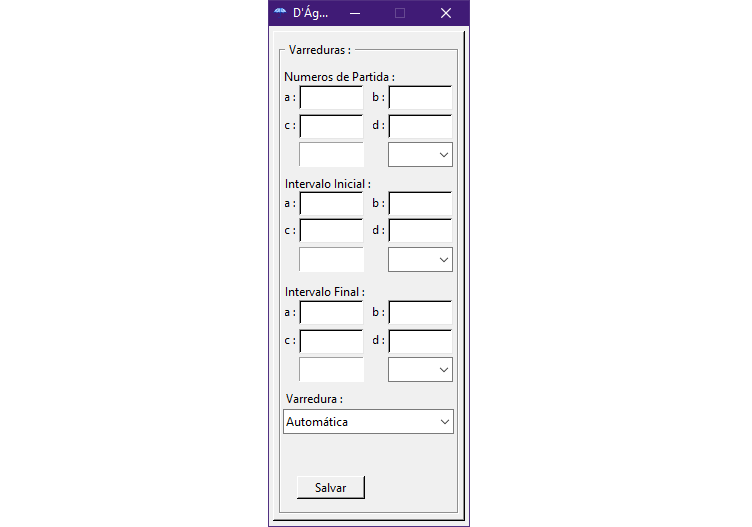
\includegraphics[width=.7625\linewidth]{figuras/varreduras.png}
	\caption*{\textbf{Fonte:} De autoria própria (2023).}
	\label{fig:figuras/varreduras.png}
\end{figure}

A última ferramenta é a de \textbf{Ajuda}, e nela tem-se os itens "Estudo" que aborda o presente trabalho como visto na Figura 5.7, "Ferramenta" que explica como funciona a inserção de dados e cálculos, observada na Figura 5.8, e "Siglas" que trata das abreviaturas visível na Figura 5.9.\bigskip

\begin{figure}[!ht]
	\centering
	\caption{Estudo da ferramenta Ajuda.}
	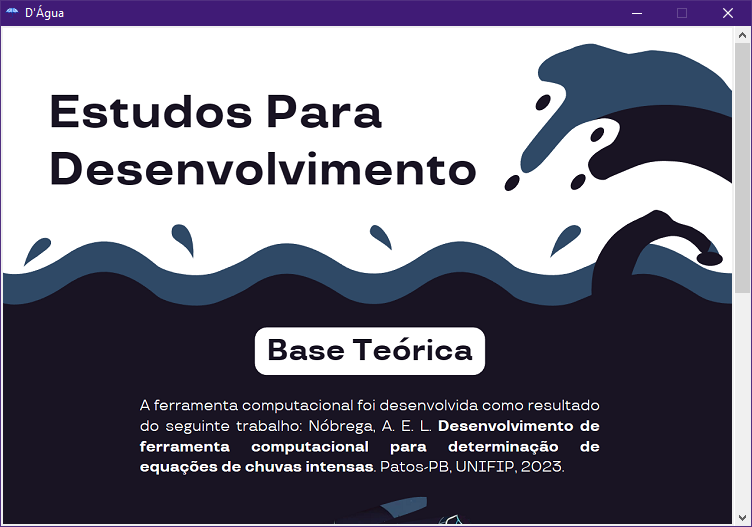
\includegraphics[width=.7625\linewidth]{figuras/estudo.png}
	\caption*{\textbf{Fonte:} De autoria própria (2023).}
	\label{fig:figuras/estudo.png}
\end{figure}

\begin{figure}[!ht]
	\centering
	\caption{Ferramenta da ferramenta Ajuda.}
	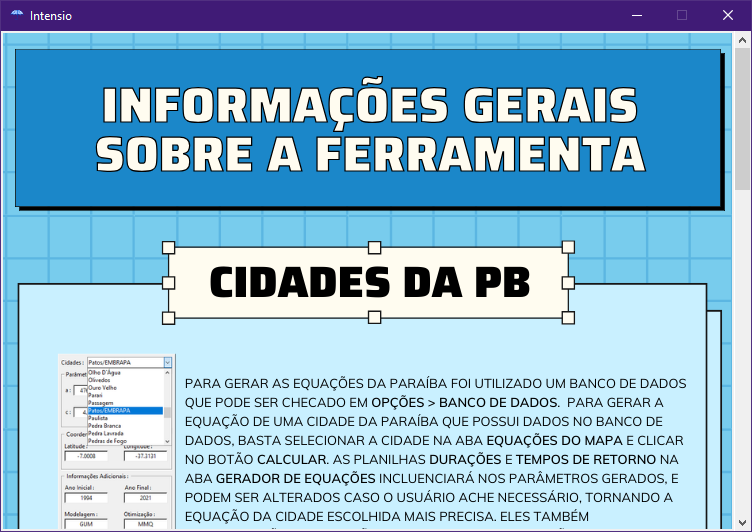
\includegraphics[width=.7625\linewidth]{figuras/ferramenta.png}
	\caption*{\textbf{Fonte:} De autoria própria (2023).}
	\label{fig:figuras/ferramenta.png}
\end{figure}

\newpage

\begin{figure}[!ht]
	\centering
	\caption{Siglas da ferramenta Ajuda.}
	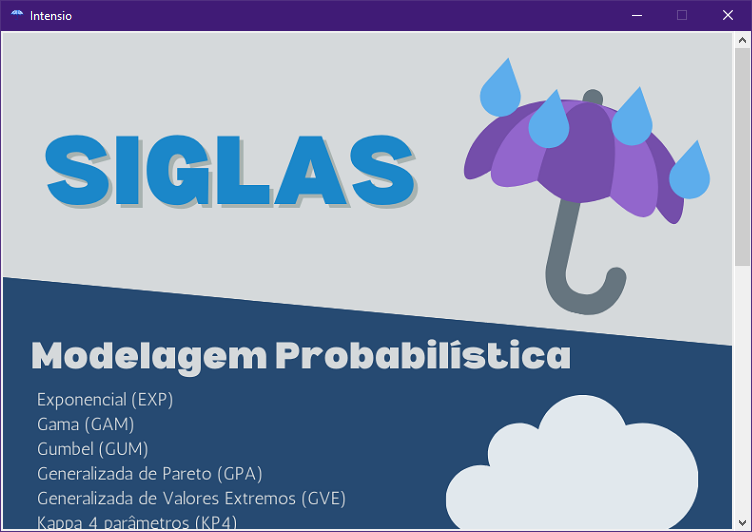
\includegraphics[width=.7625\linewidth]{figuras/siglas.png}
	\caption*{\textbf{Fonte:} De autoria própria (2023).}
	\label{fig:figuras/siglas.png}
\end{figure}

\section{VALIDAÇÃO DAS EQUAÇÕES GERADAS}

A validação das equações se trata da análise da acurácia destas, após geradas. Sempre que o usuário submeter dados, escolher uma coordenada do mapa ou cidade da lista e calcular os parâmetros da equação IDF, será gerado um relatório que pode ser acionado ao clicar no botão de mesmo nome, e pode ser visto tanto na Figura 5.1 como na Figura 5.2. Neles, estão contidos os testes de NS e RMSE, que informam o quão precisos estão os parâmetros em relação às curvas IDF qual eles foram calculados.

É importante notar que cada equação será analisada individualmente, cabendo ao calculista decidir de acordo com os testes feitos, se ele está satisfeito com a precisão dos parâmetros gerados. Outra observação importante a se fazer é a de que, os testes de acurácia analisam apenas se os parâmetros calculados estão precisos em relação aos dados observados, logo, cabe ao usuário discernir se as séries históricas que ele está informando representam bem a realidade.

É possível salvar o relatório gerado em um arquivo de texto, que informa a representação da equação IDF, um resumo de todo o processo de cálculo feito junto de todas as variáveis calculadas, e uma tabela com intensidades calculadas a partir da equação gerada, utilizando as durações e tempos de retorno informados no início do cálculo. Visualiza-se a página do relatório na Figura 5.10.

\newpage

\begin{figure}[!ht]
	\centering
	\caption{Relatório dos parâmetros da equação IDF.}
	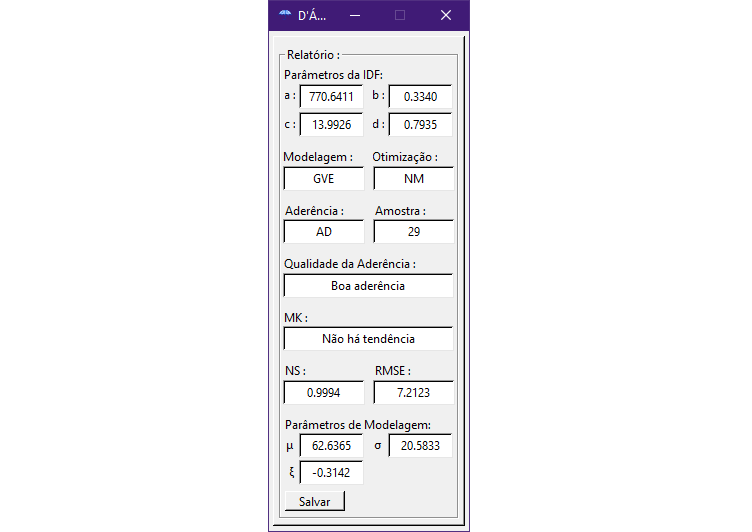
\includegraphics[width=.7625\linewidth]{figuras/relatorio_de_equacoes.png}
	\caption*{\textbf{Fonte:} De autoria própria (2023).}
	\label{fig:figuras/relatorio_de_equacoes.png}
\end{figure}

Existe também um relatório para o tratamento de dados que é acionado pelo botão de nome similar visto na Figura 5.3. Nele consegue-se analisar a quantidade de dias totais e faltantes, além da porcentagem de erros obtido, e permitido de acordo com o limiar de falhas informado. Também é possível salvar esse relatório em um arquivo de texto que contém as informações do tratamento de dados e uma tabela com as precipitações máximas diárias anuais geradas. Observa-se a página do relatório na Figura 5.11.\bigskip

\begin{figure}[!ht]
	\centering
	\caption{Relatório de falhas do tratamento de dados.}
	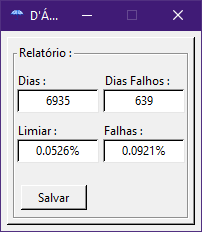
\includegraphics[width=.21\linewidth]{figuras/relatorio_de_falhas.png}
	\caption*{\textbf{Fonte:} De autoria própria (2023).}
	\label{fig:figuras/relatorio_de_falhas.png}
\end{figure}

\section{DISPONIBILIZAÇÃO DA FERRAMENTA}

Como resultado final, foi disponibilizado por Nóbrega (2023) o acesso ao repositório com o código fonte, e caminho para transferência do instalador da ferramenta computacional.
